\chapter{复习课教学录像研究结果及分析}


\section{总体情况}

在两节复习课中,两位教师都提前让学生绘制了本章的思维导图,课上运用课堂提问的教学方法,但是在提问数量上以及提问类型上都存在部分差异,如图~\ref{fig:1} 所示。

\begin{figure}[htbp]
  \centering
  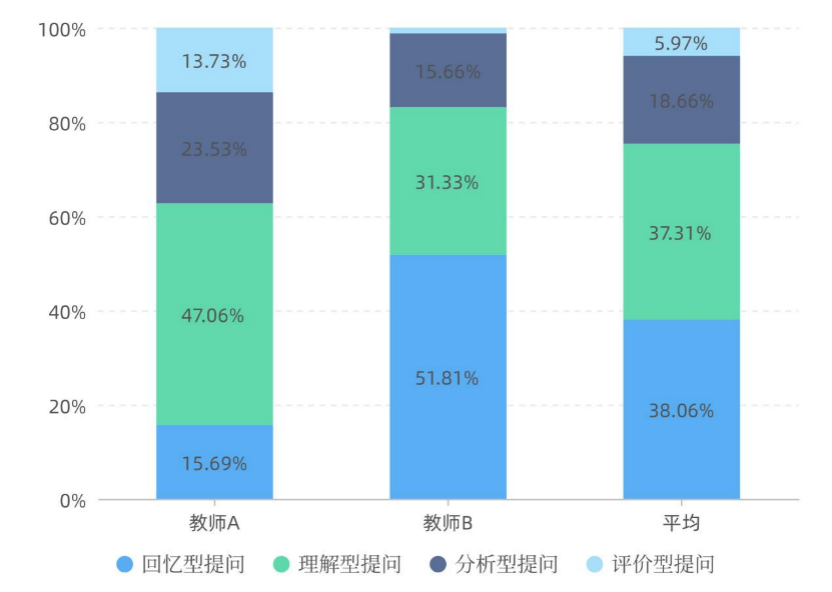
\includegraphics[width = 0.8\textwidth]{pic1.png}
  \caption{复习课两位教师不同提问类型次数的百分比比较}
  \label{fig:1}
\end{figure}

对两节课堂的提问进行统计,其中,教师A提问总数为51个,教师B提问总数为87个。本文将课堂提问分为四种类型:回忆型提问、理解型提问、分析型提问、评价型提问,其中,回忆型提问和理解型提问是低层次提问,分析型提问和评价型提问是高层次提问。教师A的低层次提问共占总提问的62.75\%,教师B的低层次提问共占总提问的83.14\%,都占总提问的大部分。其中,教师A的低层次提问中,理解型提问占总提问的47.06\%,而教师B的低层次提问中,回忆型提问占总提问的51.81\%。两位教师的高层次提问中都是分析型提问占比更大。



\section{课堂提问设计的启发}

\subsection{复习提问可适当取舍}

两位教师低层次提问的区别值得我们注意,这一差异的原因可以从教学设计中寻找到原因。

教师A在教学设计中说明,她所带领的学生已经学习了函数的概念、函数的性质,学会了研究函数的基本方法,还学习了一次函数、二次函数、指数函数、对数函数等基本初等函数模型,并且在前两章已经尝试过章末总结初步掌握了小结的方法与要点,因此本节课想通过具体问题的解决,提高学生对函数的理解、用函数处理现实问题的能力,提升对数学知识之间内在联系性的认识,增强用函数、用数学的意识。而从教师B的教学设计中可以得知,她所带领的学生初次尝试总结一章的学习内容,学生虽然对每个知识点已经有了一定的掌握,但是比较凌乱,没有形成体系,希望通过章节复习课帮助学生梳理知识,建构知识网络。

由此可以注意到,复习课的教学目的分为两种,一是检测学生对旧知的掌握程度,二是借复习引出新的知识,承上启下。两种教学目的没有高下之分,适合学生的便是好的。对于教师A所带的学生,从课堂一开始的学生展示环节中可以看出,各组学生在课下绘制思维导图的过程中,已经比较充分复习过了本章的基础知识点,课上便不需要再次由老师带领复习。而对于教师B所带的学生,课堂展示环节时教师便指出了思维导图的部分错误,因此后续的基础知识复习是十分有必要的。在进行课堂提问设计时,应当从学生学情出发。即使同为复习课,根据学生学习情况的不同,也要制定合适的复习目标。


\subsection{高层次提问应适合学生最近发展区}

两位教师在进行高层次提问时都比较保守,但是教师A的高层次提问是非常有借鉴意义的,例如“请你分享一下为什么你们小组推荐这位同学的思维导图呢?”、“如果让你选择,这两个模型,你会选哪一个?为什么?”。教师A的高层次提问都设置在小组讨论环节后,或者是对问题深度分析后提出的,给予学生充分的思考时间,此时学生已经具备回答高层次问题的能力,这样的问题设置符合学生的最近发展区。

在进行高层次提问时,应当层层铺垫,给予充分思考讨论时间,给学生搭好“梯子”,使得高层次提问也能位于学生的最近发展区,而不是突然提出高深问题,使得学生不知所云,无从下手。


\subsection{以启发性提问作为评价语言}

学生回答问题时,思维不一定清晰流畅,语言组织能力或许不足以准确表达自己的思路,此时教师应当及时利用课堂提问这一教学手段加以提醒,以“提问”代替“纠错”,使得学生自己进行补充或纠正。例如在教师A的课堂中,一位学生分享解题思路时说的是“我们可以先画出它的图像”,教师A追问“谁的图像”、“图像怎么画”,学生立刻就说出了具体的函数,以及画图思路。对于同一问题,另一同学提出了不同的思路,她指出可以画另一个函数图像,教师A也追问道:“这个函数是怎么来的?”,学生便介绍了自己的解题思路,由因到果,环环相扣,极好地锻炼了学生的思维以及语言表达能力,同时也能让听的同学豁然开朗,毕竟在课堂上,每位学生的参与都是十分重要的。即使在这段对话过程中,看似是教师与某位学生一对一的交流,但是要让班级的其他同学都参与到这个思考过程中,深入理解问题。

在数学学习过程中,许多学生往往认为数学是“玄学”,他们总认为教师所想到的方法是凭空产生的,自己根本想不到。讲解的时候,若教师没有解释清楚思路的来源,同学便会觉得这数学解题思路仿佛是腾空出世的孙悟空一般,可遇而不可求,长此以往,学生对于数学学习便更会失去信心与动力,十分不利。因此,对于解题思路的讲解更要做到“刨根问底”,启发性追问便是很好的辅助手段。


\subsection{复习课需借助课堂提问辅助学生总结}

教师A与学生研究方程 $x |x - 2| + b = 0 (b \in \mathbb{R})$ 根的个数问题时,学生们提出了四种方法,随后教师A带领学生总结这类题型的解题思路与方法,一开始学生难以总结,所以教师A接连提出以下几个问题:先从共同点和不同点入手吧。其中,这么多种方法,共性是什么?这个方法,和其他方法是不是不太一样?他用的是什么方法?那么其他三个方法呢?那么数形结合为什么会出现三个不一样的方法呢?这些问题能够很好地帮助学生梳理易掌握的知识与方法,建立起自己的知识框架。



\section{课堂提问设计的误区}

\subsection{课堂提问表面化}

教师A的课堂上,各小组分享完思维导图后,教师A提问:“那么我们以后小结的时候,应当往哪些角度去小结呢?”此时教师手指黑板板书,引导学生念出来,因此上文所提到的问题,看似是分析型问题,实际是回忆型问题。研究超速车辆案例时,教师A提问:“比如说,当交通事故出现时,我们首先要做什么?”但PPT上已展示出答案。同样的提问误区也出现在教师B的课堂中。某位学生分享完思维导图后,教师B提出了这样一个问题:"她的知识结构图其实有点小问题,在哪里?",而后教师B立刻指出错误所在,并未让学生实际作答。本可以让学生来评价,进行高层次提问,却由教师先行评价,不仅降低了提问层次,更使得提问浮于表面。在某位学生进行归纳后,教师B问全班同学:她归纳的好不好?这看似是评价型问题,但没有要求学生说出好与不好的依据所在,仅仅一个“好”字带过,浪费问题。在一节知识基础复习后,教师B提问:以上这些公式都是在谁的基础上推导出来的?这本是一个理解型问题,学生不仅需要记住以上的公式,还需理解公式的推导过程,但是教师B早已在课件上展示答案,使得这问题在课堂中轻飘飘一笔带过。除此之外,教师A的课堂提问中有5个问题是教师自问自答,教师B的课堂提问中有6个问题是教师自问自答。

不论是黑板板书写好答案,还是PPT课件提前展示答案,都说明许多提问教师早已设计好回答,更有教师以“自问自答”方式处理课堂提问,说明教师的课堂提问是以引导学生跟随教师思维为目的,并没有将学生个体的思考与理解放在主体地位。这样的课堂看上去整堂课都在提问,学生也积极回答,但细想一下,少有学生思维活动在其中,无从体现学生在学习中的主体地位,与“满堂灌”的教学方式并无差异,仍旧是机械的填鸭式教学。


\subsection{提问语言欠缺准确性}

教师提问一定要注意语言的准确性,让学生明确思考方向,一旦沟通过程出现些许偏差,教师应补充说明,不要让语言表达成为数学学习上的阻碍。在这一点上,两位教师都有不足之处。教师A带领学生探讨“超速车辆车祸”问题时,有一环节是交警可以根据车速与刹车距离的关系式推算出车祸发生时车辆的时速,教师A问道:“如果你是交警,没有这个函数关系式,你会获取吗?打算怎么获取?”学生认为可以现场真实车辆模拟从而得到结果,教师A反问:“假如肇事司机是在飙车,那你也要让模拟人员飙车吗?我们要探究的是,这个120具体数字怎么得来?”这位老师是希望学生明白我们可以利用函数模型来推测车辆时速,但是语言表述不明确,导致这一阶段花费了较多时间才使得学生明白老师的意思,这是我们在教学过程中应当规避的。教师B带领学生研究一组函数图像时,提问:“它的规律是?”函数图像所能体现的规律数不胜数,学生根本不知道教师问的是那一方面的规律,也就无人作答,课堂气氛一下子冷却下来。教师B意识到这一点后,及时补充提问:“这一组函数的单调性与底数有什么关系呢?”这才使得学生理解。


\subsection{提问对象不合理}

教师B的课堂提问往往直接面向单个学生,并且是提出问题后立刻点名某一学生回答问题,这样的课堂提问太像一对一谈话,重点是解决问题,而不是对问题的探索过程。这样的提问方式,会给予部分学生偷懒的机会,因为教师只会和被点名的学生沟通,那么班级里的部分其余同学就会认为事不关己,高高挂起,直接放弃对问题的思考,这对教学是极为不利的。但这并不代表课堂提问不能点名回答问题,而是在这一过程中,应当使大部分学生都能积极参与问题的探索过程,即使最后回答问题的只是个别同学,也要让大部分同学都处于思考状态。
